% \chapter{Introduction}
% \label{introduction}


% \begin{itemize}
    %     \item Chiral review \cite{epelbaum_frontiers}
    
    %     \item Weinberg \cite{WEINBERG1990}\\
    %         Weinberg \cite{WEINBERG1990} suggested using a most general Lagrangian
    %         satisfying spontaneously broken chiral symmetry and other symmetries and
    %         evolving pions together with low-energy nucleons.
    
    %         \item Epelbaum \cite{epelglockle98, epelglockle2000, epelglockle2003}
    %     \item The newest chiral force \cite{reinkrebs2018} 
    
    %     \item Arenhovel \cite{ArenhovelPhotodisint1991}
    %     \begin{itemize}
        %         \item He used different currents (`names, types')
        %         \item Approaches
        %     \end{itemize}
        % \end{itemize}
% \section{Historical overview}
        
% In the second half of XX century physical society faced
% a problem of describing low-energetic nuclear reactions.
% \gls{qcd} is hardly applicable here as it is nonperturbative 
% at low energies what complicates a lot search for the solutions \cite{Machleidt2011}. 


% \printglossary[type=\acronymtype]
% \printnoidxglossary[type=acronym]

\chapter{Introduction}

% \begin{itemize}
%     \item Why we study few nucleon systems
%     \begin{itemize}
%         \item Strong interactions (2N and 3N force investigation; QCD, relativistic effects)
%         \item Electro-magnetic processes (electrons-, photons-induced reactions) (Arenhovel did ...)
%         \item Weak interactions (neutrons)
%     \end{itemize}

%     \item Nuclear forces used in the thesis
%     \begin{itemize}
%         \item AV18
%         \item Chiral (scs, sms; difference between chiral models; regularisation problem)
%     \end{itemize}

%     \item Currents used in the thesis (regularisation of currents to be done)
    
%     \item Formalism \& numerical methods
%     \begin{itemize}
%         \item Lippman-Schwinger eq
%         \item Schrodinger eq for deuteron; wave functions (sms) for deuteron - figures, binding energy
%         \item Three body: Fadeev eq. for bound (He3, H3) and scattering states
%         \item Siegert theorem ?
%         \item Partial wave decomposition, states ($pq\alpha$), Jakobi momenta;
%         operators in PW decomp. (current); Mathematica for PW
%         \item Theoretical uncertainties: truncation error, cut-off dependency, chiral order dependency
%     \end{itemize}

%     \item Results (\textbf{find everything what I have calculated: all processes and energies} )
%     \begin{itemize}
%         \item H2 photodisintegration
%         \item He3 and H3 photodisintegration
%         \item Pion capture
%     \end{itemize}

%     \item Summary
    
%     \item References
% \end{itemize}

\subsection*{Why we study few nucleon systems}

The study of light nuclei and their reactions has been serving as an easy way to investigate particles in nuclei and
the forces between them for decades. A convenient way to proceed may be to study the interaction of a nucleus with
other nuclei, particles, or electroweak probes such as electrons, photons, muons, pions, neutrinos, and hyperons.
In most cases, study of elastic or inelastic scattering is possible. This can be done either theoretically or by
performing relevant experiments to test if the theory works. It should be taken into account that nuclear 
interactions may be
caused by different fundamental forces, including strong, weak, or electromagnetic
interactions. This depends on the type of particle being scattered and the target of the reaction
and requires different theoretical approaches.
Of course gravitational force is also in the game but due to its weekness it is 
usually omitted in the nuclear physics. 

In the past many experimental efforts have been undertaken and
experimentalists have been interested in electromagnetic reactions involving light nuclei for decades.
There are experimental data from the second half of 20th century 
(e.g. \cite{Skopik1974, Liuexp68, Kose1969MeasurementsOT, Kamae}) which are still 
useful for comparing theoretical predictions with experimental measurements.    
There are several facilities providing sources of gamma rays (both low- and high-energy)
and other particles that have been operating for decades and still enable experiments to be conducted.
Let us mention here such facilities as TUNL with HI$\gamma$S \cite{TUNL, TONCHEV2005170}, MAMI \cite{MAMI}. 
% NIKHEF \cite{NIKHEF} and others.

To accurately describe nuclear reactions, two important components of the Hamiltonian must be considered.
They are nuclear interactions and nuclear currents.
First of all, various nuclear forces may act on
the particles.

The strong nuclear force acts inside the nuclei and, among others, bound neutrons 
and protons together. The description of strong interactions is extremely
difficult as it deals not only with the nucleons themselves, but also with their constituents: quarks
and gluons. \gls{qcd} is a modern theory
describing strong interactions, but, at the moment,
it is not applicable at low energies (e.a. at $Q^2 \lesssim 1 GeV^2$).
In such situation various approaches are emerging.
The most advanced are the
chiral effective theory and lattice calculation \cite{IOFFE2006232, BEANElaticce, Machleidt2011}.
In this work we will use results of the first approach
and corresponding model is described in Sec.~\ref{sec:formalism}.

Study of three- (and more) nucleon systems showed that
the strong \gls{2n} force is not efficient in describing
$N>2$ systems, thus a 3N force was introduced. The first applications of such
a force showed that it brings a
sizable contribution to observables and cannot be ignored \cite{GLOCKLE1982343}.
The contribution of the 3NF can be examined by
comparing binding energies of light nuclei calculated with
and without this part of Hamiltonian with respect to experimental values.

For example, the binding energy for $^3$H calculated with the \gls{av18} \gls{2n} potential 
without 3NF amounts to
$E_b(^3\mathrm{H}) = \SI{-7.628}{\mev}$ \cite{NoggaAV18}. There are different models that might add a 3NF
contribution to \gls{av18} (or other potentials). Using the Tucson-Melbourne (TM) model \cite{Tucson-Melbourne}
results in $E_b(^3\mathrm{H}) = \SI{-8.478}{\mev}$, and Urbana IX \cite{Urbana3NF} 3NF provides us with
$E_b(^3\mathrm{H}) = \SI{-8.484}{\mev}$. Looking at the experimental value $E_b(^3\mathrm{H}) = \SI{-8.482}{\mev}$,
it is clear that the 3NF contribution makes the prediction much closer to the measurement.
Nevertheless, the parameters of the UrbanaIX
3NF were fitted to the experimental value for $^3\mathrm{H}$, so there is no surprise in good agreement.

However one can also check the binding energy for other nuclei, which were not used for the fitting.
The 2NF binding energy for $^3$He
(calculated with \gls{av18}) is $E_b(^3\mathrm{He}) = \SI{-6.917}{\mev}$. TM contribution makes it
$E_b(^3\mathrm{He}) = \SI{-7.706}{\mev}$, Urbana IX gives $E_b(^3\mathrm{He}) = \SI{-7.739}{\mev}$, while the
experimental value is $E_b(^3\mathrm{He}) = \SI{-7.718}{\mev}$. One can see the importance of 3NF
contribution also for the $\alpha$-particle's ($^4\mathrm{He}$) binding energy:
\gls{av18} alone gives
$E_b(^4\mathrm{He}) = \SI{-24.25}{\mev}$, while \gls{av18} + TM leads to \SI{-28.84}{\mev},
\gls{av18} + Urbana IX delivers $E_b(^4\mathrm{He}) = \SI{-28.50}{\mev}$,
and the experimental value is \SI{-28.30}{\mev}\cite{NoggaAV18}.

Whereas the first applications included only early simplified "realistic" 3N potential, the latter
investigations, based on more advanced models, fully confirmed this statements \cite{StoksPhysRevC49, AV18Wiringa}.
Within new models the four-nucleon (4N) interaction was constructed to improve description of
$^4\mathrm{He}$ \cite{NoggaPhysRevLett}.
Broader discussion of nuclear forces used in this thesis is given below.

Electromagnetic force appears between charged particles like protons, electrons or pions.
That force acts also between charged particles and photons, so 
in photon- and electron- scatterings on the nuclei 
it is a necessary component of a description.
However, electromagneticinteraction between particles manifests only at very 
low energies or for specific kinematic configurations with two
photons having approximately equal momenta.
Thus it rather is being skipped in lowes-order analysis.

The main conribution of electromagnetic interaction 
to disintegration processes in hand is due to the current's operator
describing photon-nucleon vertex.
The structure of the electromagnetic current have been investigated
in many works by numerous groups \cite{Carlson1997} but it was 
H.~Arenh\"{o}vel who performed study of nuclear electromagnetic
current in few-nucleon sector.
His long-term research, reviewed in \cite{ArenhovelPhotodisint1991}
% in his works
% \cite{Wilbois1993, ArenhovelLeid1995, ArenhovelLeid1998, Arenhvel2004} 
demonstrated various theoretical models applied to the deuteron photodisintegration.
He analyzed among others a nonrelativistic potential model,
a relativistic impulse approximation, and a relativistic meson-exchange model.
These models were used to calculate the differential cross section and various
polarization observables, which describe the probability
of the process occurring at different scattering angles, photon energies spin directions etc.

The calculated cross sections were then compared to experimental data, and it was
found that the relativistic meson-exchange model provided
the best agreement with the data at photon's energies up to $E_\gamma = \sim\SI{100}{\mev}$.
At higher energies agreement is presented but is getting worse.
This model includes the exchange of virtual mesons
between the interacting particles, which accounts for
the strong and electromagnetic forces between them.

Overall, Arenh\"{o}vel demonstrated the importance of including both strong interaction
and electromagnetic current operator in a description of the deuteron photodisintegration process,
and highlighted the need for accurate theoretical models to interpret experimental data.

% Arenh\\"{o}vel \cite{ArenhovelPhotodisint1991} 
% studied electromagnetic process - deuteron photodisintegration,
% applying different approaches and comparing the results with
% experimental data.


% The electromagnetic current operator for a few-nucleon system has both one- and many-body contributions, which
% can be denoted as $j_\mu^1$, $j_\mu^2$, and $j_\mu^3$, respectively. The leading one-body contribution,
% $j_\mu^1$, represents the photon's interaction with a single nucleon. The many-body contributions are known as
% meson exchange currents (MEC), which arise due to the meson-exchange picture of the nucleon-nucleon (NN)
% interaction. The photon can couple to mesons exchanged between two nucleons, leading to two-body contributions to
% the nuclear current.

% The necessity of introducing the MEC arises from the continuity equation, which requires the inclusion of
% two-body interactions in the Hamiltonian. The momentum and isospin-dependent terms in $V$ require the
% introduction of two-body MEC. Similarly, the inclusion of the three-body force into the Hamiltonian requires the
% existence of three-body contributions to the nuclear current. However, the effects of the three-body MEC are
% likely negligible in the low-energy region. Therefore, we will only consider one- and two-body currents.

% The nuclear one-body current is constructed based on the electromagnetic current for a Dirac particle. To account
% for the extended structure of nucleons, form factors are introduced. Since we use nonrelativistic wave functions,
% we need to use nonrelativistic currents. The currents used in the thesis are described in Sec.~\ref{sec_current}.

The weak force is of great importance in the study of nuclear processes. One of the main roles of the weak force is to mediate \tmp{check correction} beta decay,
which is a process in which a neutron in a nucleus is converted into a proton, emitting an electron and an antineutrino. This process plays
a crucial role in the formation of elements in the universe, as it allows for the conversion of neutron-rich isotopes into more stable,
proton-rich isotopes. Additionally, the weak force plays a role in neutrino interactions with matter, which are of great interest in both
astrophysics and particle physics. In nuclear physics, weak interactions can also play a role in the decay of unstable nuclei, the
production of neutrinos in nuclear reactions, and the scattering of neutrinos off nuclei. The study of weak interactions is therefore an
essential component of the overall understanding of nuclear physics and the behavior of matter on the subatomic scale.
However, in the thesis we stick up with electromagnetic processes.


\subsection*{Models of strong interaction used in the thesis}

In order to model the nuclear potential, physicists often use phenomenological
or semi-phenomenological approaches. It allows them to combine
theoretical knowledge about the studied processes and experimental findings.

\tmp{?more}
Among many of such models, the \gls{av18} \cite{AV18Wiringa} force is one of most
advanced and therefore is used in current thesis.
In order to construct the \gls{nn} force, authors combine
% analytical electromagnetic and 
one-pion-exchange part
with phenomenological one and supplement them by electromagnetic corrections.
Free parameters were fitted to
the Nijmegen partial-wave analysis of $pp$ and $np$ data \cite{NijmegenPhysRevC.48.792}. 
Authors showed, that the \gls{av18} potential delivers good 
description of nucleon scattering data ($\chi ^2/data = 1.08$ for around \num{4000} $pp$ and $np$ scattering datasets) 
as well as deuteron properties (estimated binding energy is \SI{2.2247(35)}{\mev} vs experimental \SI{ 2.224 575(9)}{\mev}).

Weinberg's idea of using chiral symmetry to describe nuclear interactions at low
energies was first introduced in his papers published in 1990 and 1991 \cite{WEINBERG1990,WEINBERG1991}.
In these papers, Weinberg argued that the low-energy dynamics of nucleons
could be described using a chiral Lagrangian, which is the most general
Lagrangian consistent with chiral symmetry and its spontaneous breaking.
This Lagrangian is expressed in terms of nucleon and pion fields,
which are the degrees of freedom that become relevant at low energies.

The chiral Lagrangian is the starting point for the development of
the \gls{ceft}, which has become one of the
most advanced approaches to low-energy nuclear physics \cite{EpelHam2008}.
The use of the \gls{ceft} allows (at least in theory) for the calculation of nuclear properties
and reactions in a model-independent way.
It is also possible to
quantify the uncertainties associated with the calculation. One of the
key features of the \gls{ceft} is that it allows for the construction of
a nuclear potential, which can then be used in relevant formalisms, e.g. to solve the Schr\"odinger
equation and to obtain bound and scattering states properties. The accuracy of the
potential can be systematically improved by including higher-order
terms in the chiral expansion, which leads to a better description of
experimental data.

% In the early 1990-ies Weinberg \cite{WEINBERG1990,WEINBERG1991} introduced 
% an idea of using the most general Lagrangian
% satisfying assumed symmetry principles and in particular
% spontaneously broken chiral symmetry to 
% describe nuclear interactions at low energies.
% This idea together with \gls{eft} of \gls{qcd} 
% led to the development of the \gls{ceft}
% % a Chiral effective field theory ($\chi$EFT)
% which nowadays has become one of the most advanced approach to
% low-energy nuclear physics. While in \gls{ceft} it is possible to study processesor bound states directly,
% it is also possible to describe nuclear potential, which can be next used in quantum equations,
% e.g. Schr\"odinger equation.
 
% For the \gls{eft} it is very important to 
% define a quantity, which powers will determine a perturbation order.
% The basic idea
% of \gls{ceft} is to construct a systematic expansion of the nuclear
% interaction in powers of the small parameter $Q/\Lambda_\mathrm{ch}$,
% where $Q$ is a typical momentum or energy scale of the process under
% consideration and $\Lambda_\mathrm{ch}$ is the chiral symmetry breaking
% scale, which is around \SI{1}{\giga\electronvolt}.
In the \gls{ceft} there are two natural scales: so-called soft scale $Q \sim M_\pi$  -
the mass of pion and the hard scale -
$\Lambda_\chi \sim \SI{0.7}{\gev}$ - the chiral symmetry breaking scale.
The ratio between these two scales $Q/\Lambda_\chi$
is being used as an expansion parameter in  \gls{ceft} with power
$\nu$: $\left(Q/\Lambda_\chi\right)^\nu$.
\footnote{Note that exact values of some parameters are still under discussion \cite{Epelbaum2004}. We follow here approach proposed by E.Epelbaum and collaborators, see e.g. \cite{reinkrebs2018}}

Possibility of deriving nuclear potential is an important feature of \gls{ceft}.
The potential, as occurs in Lagrangian, is a perturbation expression of the same parameter $Q/\Lambda_\chi$.
Considering so-called irreducible diagrams (which cannot be split
by cutting nucleon lines), Weinberg \cite{WEINBERG1990,WEINBERG1991}
came to the expression for the powers $\nu_W$ of such diagrams

\begin{equation}
    \nu_W = 4 - A - 2C + 2L + \sum_i \Delta_i,
    \label{powers}
\end{equation}
where $i$ specifies a vertex number and

\begin{equation}
    \Delta_i \equiv d_i + \frac{n_i}{2} - 2.
    \label{Delta}
\end{equation}

In \eq{powers} $C$ is a number of pieces which are connected, $L$ - the number of loops in the graph
and $A$ is a number of nucleons in the diagram.
In \eq{Delta} $n_i$ is a number of nucleon field operators and $d_i$ - the number of insertions
(or derivatives) of  $M_\pi$.

The further analysis of \eq{powers} revealed some problems which occur 
for particular values of parameters in the equation, namely negative values of $\nu_W$ 
are possible while the order has to take integer values from 0 to infinity.
In order to deal with that, \eq{powers} 
was slightly modified by adding $3A - 6$ to it  \cite{Machleidt2011, EPELBAUM2006_PROGRESS}:

\begin{equation}
    \nu = \nu_W + 3A  - 6 = -2 + 2A - 2C + 2L + \sum_i \Delta_i.
    \label{powers_corrected}
\end{equation}

That convention above is widely used and we will also stick to it as well.

In \gls{ceft} the first order, "leading order" ($\nu=0$) is followed 
by the next-to-leading order ($\nu=2$)
\footnote{The contributions to the potential at order $\nu=1$ completely vanish due to parity and time-reversal invariance,
so the next-to-leading order stands for the second order ($\nu=0$) of expansion.},
 the next-to-next-to-leading order ($\nu=3$) and so on.
 At each chiral order, new interaction diagrams complete the potential.
 There are only two diagrams at \gls{lo}: one is a contact term
 and the other one
 is a one-pion exchange, see \fig{chiral_diagrams}. Both diagrams reflect only 2NF.
 The same is for diagrams at \gls{nlo}, where more contact terms occure together with two-pion 
 exchange topologies. Each subsequent order includes more and more sophisticated diagrams
 describing nucleons interaction
 via multiple  pion exchanges and various contact verteces.
 3NF appears for the first time at \gls{n2lo}
 while 4NF contributions start from \gls{n3lo}.
 This scheme establishes for the first time a systematic
way to include all the contributions to a strong nuclear force
 starting from the simplest diagrams at LO and gradually
adding more and more terms. 
It is also beneficial in the way that 
one can obtain results using chiral potential at different
orders and track which one gives large or small contribution to the final prediction.
At the moment, \gls{n4lo} is the highest order at which 2N interaction has been completely derived.
Nevertheless leading F-wave contact interactions from N$^5$LO have been combined with \gls{n4lo} force
leading to the \gls{n4lo+} potential,
which is currently regarded as a best available potential on the market.
The progression of the chiral orders is reflected in a $\chi^2/data$.
Leading order results in $\chi^2/data = 73$ (with neutron-proton data with $E_{lab} = 0-100 \unit{\mev}$).
Each subsequent order has better and better results: \gls{nlo} gives $\chi^2/data = 2.2$, \gls{n2lo} - $\chi^2/data = 2.2$
and the highest, \gls{n4lo+}, leads to $\chi^2/data = 1.08$ \cite{reinkrebs2018}.
Similar progress is observed for wider energy range, e.g for $E_{lab} = 0-300 \unit{\mev}$
$\chi^2/data$ is 75, 14, 4.2, 2.01, 1.16 and 1.06
at LO, NLO, \gls{n2lo}, \gls{n3lo}, \gls{n4lo} and \gls{n4lo+}, respectively.
The proton-proton data description has similar trend, so $\chi^2/data$ is 1380, 91, 41, 3.43, 1.67, 1.00 
for the same energy bin and chiral orders. At \gls{n4lo+} $\chi^2/data$ for proton-proton data
stands similar value (close to 1) as for neutron-proton, but the convergence comes a bit later and 
leading order has way worse description.
In my work I will use chiral potentials from \gls{lo} up to \gls{n4lo+}.

\begin{figure}[h]
    \begin{center}
    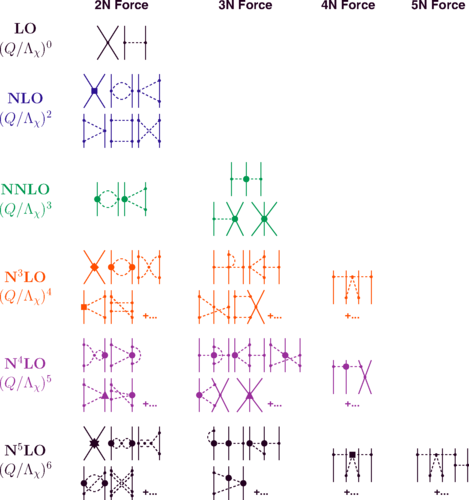
\includegraphics[width=0.6\textwidth]{Figures/chiral.png}
    \end{center}
    \caption{\tmp{Make own diagrams, e.g. with JaxoDraw or PyFeyn \cite{Entem2017}}}
    \label{chiral_diagrams}
\end{figure}

The Argonne V18 potential \cite{AV18Wiringa}, mentioned earlier, has 40 adjustable parameters,
while \gls{ceft} NN potential at \gls{n4lo} \cite{Machleidt2011} has only three\tmp{???} low-energy constants (LECs) fitted to deuteron properties.
The reduction of the number of free parameters of the \gls{ceft}-based potentials
has not only a theoretical but also a practical advantage in the studies of nuclear systems.

The general scheme outlined above was developed mainly by the Bochum-Bonn and Moscow-Idaho groups.
Both groups have similar approaches and were independently and almost simultaneously
developing their models. In 1998 Epelbaum and collaborators from the Bochum-Bonn group 
presented a first version of their \gls{nn} chiral potential \cite{EPELBAOUM1998107, epelbaum2000two}.
Developing a more and more sophisticated versions with higher chiral orders, authors presented
\gls{n3lo} potential in 2005 \cite{epelbaum2005two} which included a 3NF contributions.
They were further developing their chiral model, taking into account more Feynmann diagrams
coming to a higher chiral orders.
At some moment Bochum-Bonn goup faced with a problem of potential regularisation\cite{skibinski_3H, Witala_2014}.
Solving it was an important step and autors
where struggling with finding an appropriate
regularization method to handle the divergences that arise in the \gls{ceft} calculations.
Different techniques were applied such as the cutoff regularization and the regulator function methods.
An important point was when authors started using a semi-local regularisation 
in the coordinate space. The correspondant potential is called  the \gls{scs} potential
(semi-local regularisation in the coordinate space)\cite{Epelbaum2014SCS}, see below in Sec{\temp{??}}.
Later similar regularisation,
but done in momentum space was introduced, resulting in the most advanced chiral potential at the moment up to  
\gls{n4lo+} chiral order \cite{reinkrebs2018}: the \gls{sms}. It is developed up to \gls{n4lo+} at the moment.

On the other side of the planet, in Idaho, Machleidt and his group from Moscow(Idaho) were also developing 
a chiral interaction. Their results from 2003 \cite{Entem2003}, following with later 
investigations \cite{Machleidt2005, Machleidt2010, Entem2017} introduced very similar model
to the one from the Bochum-Bonn
group with minor technical differences.


There are a number of another attempts to construct the nuclear
potential from the \gls{ceft}.
% There are a number of another approaches within \gls{ceft} utilized.
% There are several other approaches within the framework of \gls{ceft}
% that have been utilized in nuclear physics.
M.Piarulli et al \cite{Piarulli2012,Piarulli2015} contributed
to quite similar approach, based on
the same chiral potentials but including explicitly 
$\Delta$-isobar intermadiate states 
up to the third chiral order and taking into account
sophisticated electromagnetic corrections.

Other groups try to improve already derived forces.
Let us mention here works by A.~Ekstr\"om and
collaborators \cite{ekstrom_2015, Tews_2020} who,
by using sophisticated fitting methods combined with
statistical analysis, proposed so-called optimised interaction
V$_\text{opt}$ which was proved to provide a good description
of atom properties for radii and calcium without
using 3NF.
% Ekström and collaborators developed a chiral
% effective theory for nuclear forces and currents that includes both
% nucleon and pion degrees of freedom \cite{ekstrom_2015, Tews_2020}. Their approach
% is based on a power counting scheme that separates long-range and
% short-range contributions and allows for systematic improvements in the
% calculations.

Another approach is the pionless effective field
theory, which integrates out pions and
focuses on the various types of contact
interactions between nucleons \cite{hammer_review}.
Obtained potential has a very simple form, but cannot be applied
to higher energies since pions start playing an important role
there.

Yet another promising approach is the Lattice Effective Field Theory (LEFT), which
is based on the Lattice QCD simulations of the strong
interaction. Mei\ss{}ner and collaborators have developed a chiral effective
theory for nuclear forces based on the results of lattice QCD
calculations \cite{Lande2019}. This approach has the advantage of being able
to predict the nuclear force directly from the first
principles, without the need for phenomenological input. However, currently it is limited
to small systems and low energies due to the computational
resources required for calculations.
Up to now, the relatively simple two-nucleon scattering problem
and few-nucleon bound state
have been solved within the LEFT and more complex systems are
still under attack. 
For more details please refer to
\cite{Lande2019}.


% {\color{red} Machleidt, Ekstr\"om, pion-less EFT, Lattice EFT(Mesissner), Girlanda, Piarulli}


Technically, the chiral potential may be derived both in coordinate and momentum spaces.
Nevertheless in both cases it requires regularisation which 
improves potential behavior at small distances or at high momenta,
which allows to avoid infinities. 
% cuts 
% low coordinate values in order to avoid infinities 
% or high momentum values. 
The \gls{sms} potential is being regularized semilocally. 
It means that  local or nonlocal regularisations
are being applied for different parts of the potential.
% and later in \cite{Entem2017, Epelbaum2014SCS}
In \cite{Entem2003, epelbaum2005two} the non-local regulation scheme 
was applied to both short- and long-range parts
 of the potential while in the next model \cite{Entem2017, Epelbaum2014SCS}
 it affected only a short range part. 
This regularisation is applied directly to the potential matrix elements 
in the coordinate space:

\begin{equation}
    V_\pi(\vec{r}) \rightarrow V_{\pi,R} (\vec{r}) = V_\pi (\vec{r}) \left(1 - \exp(-r^2/R^2 )\right),
    \label{scs_regulator} 
\end{equation}
or in the momentum space

\begin{equation}
    V_\pi(\pvec{p}, \vec{p}) \rightarrow V_{\Lambda} (\pvec{p}, \vec{p}) = 
    V_\pi (\pvec{p}, \vec{p}) 
    \exp\left[-(p^\prime/\Lambda)^{2n} -(p/\Lambda)^{2n} \right],
    \label{sms_regulator} 
\end{equation}
where the cutoff R was chosen in the range of R = 0.8, ..., 1.2 \unit{fm},
$\Lambda = \frac{2}{R}$ and $n$ being adjusted with respect to the considered chiral order.
For specific case of the \gls{sms} force $\Lambda = \SIrange[range-phrase=-]{400}{550}{\mev}$ and $n=3$.

The other way of regularisation, the local one, is applied to the propagator operator,
already during the derivation of potential. Namely, the Gaussian form factor $F(\vec{l}^2)$ is being used
to reduce pions with higher momenta:

\begin{equation}
    \int_{-\infty}^{\infty} \frac{\rho(\mu^2)}{\vec{l}^2 + \mu^2} d\mu^2 \rightarrow 
    \frac{F(\vec{l}^2)}{\vec{l}^2 + \mu^2}
\end{equation}
with

\begin{equation}
    F(\vec{l}^2) = e^{-\frac{\vec{l}^2 + M_\pi^2}{\Lambda^2}},
    \label{regulator}
\end{equation}
$M_\pi$ is an effective pion mass, $\Lambda$ - a cutoff parameter and $l$ is a four-momentum of the exchanged pion.
\tmp{Further $\mu$ is a ...}
The form factor (\ref{regulator}), being used together with Feynman propagator,
ensures that long-range part of the forces has no singularities. 

The cut-off parameter $\Lambda$ is not fixed and usually calculations
are being performed for its different values. The comparison
of such results may reveal stronger or weaker dependance and in a perfect
case, which is expected at $\nu >> 1$, one will come up with such a potential, were the cut will
not affect results at all. One of aims of my thesis is to test how big cut-off dependency
of predictions is
observed for the best currently available forces (\gls{scs} and \gls{sms}). 
To illustrate a cutoff dependancy of the potential, in \fig{potential_cutoff} 
I show values of the matrix elements for 2N $\matrixel{p}{V}{p^\prime}$ potential $^3S_1-^3D_1$
as a function on the momentum $|\vec{p}|$ with fixed value $|\pvec{p}|$=\SI{0.054}{fm^{-1}}.
Please note, that relatively strong dependancy of specific matrix element of the potential
is not always leading to a strong dependancy of observables, as 
observables comprise contributions from many matrix elements.



\begin{figure}[htb]
    \begin{center}
    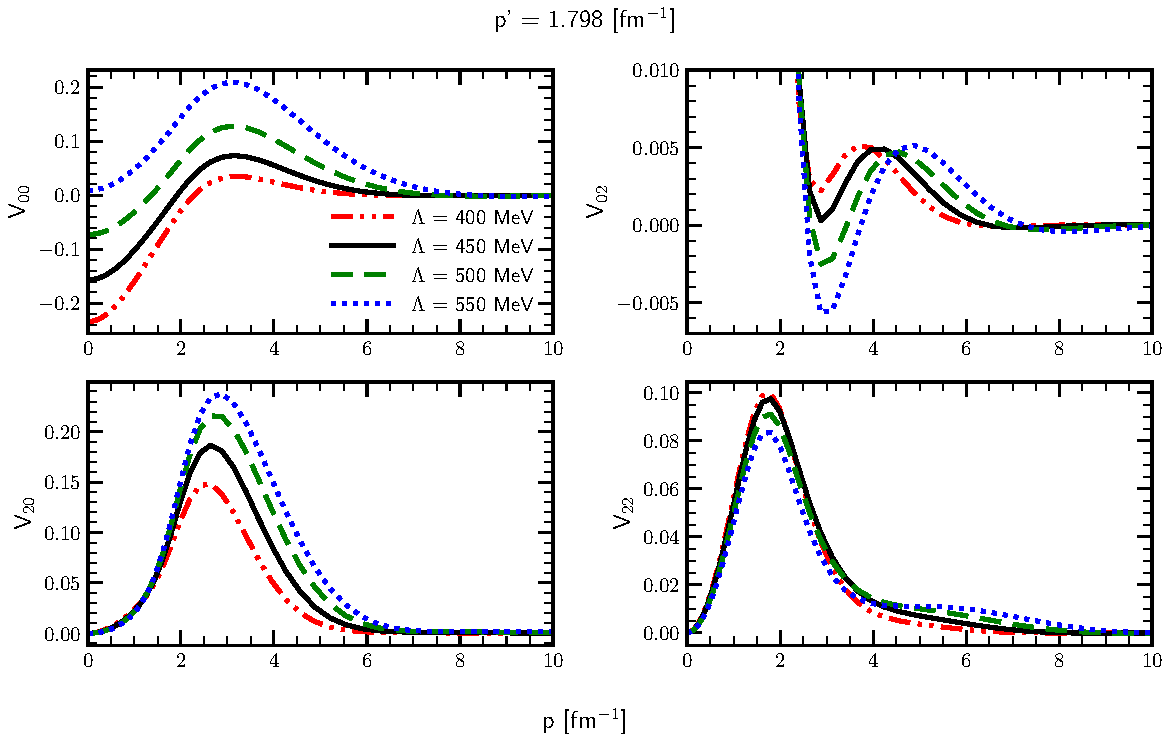
\includegraphics[width=0.95\textwidth]{PlotData/Deuteron/WAVEFUNC/potential_pp1.798.pdf}
    \end{center}
    \caption{Matrix elements $\matrixel{p}{V}{p^\prime}$ of the potential in
    coupled partial waves $^3S_1 - ^3D_1$ as a function on the momentum $p$ with fixed
    value of the momentum $p'=\SI{1.798}{fm^{-1}}$. Potential element $V_{ll'}$
    is taken between two states with angular momenta  $l$ and $l'$ where $l=0$
    stands  for $^3S_1$ state and $l=2$ - for $^3D_1$. 
    }
    \label{potential_cutoff}
\end{figure}



% The potential may be transformed from coordinate to momentum space (or vice versa),
% but it is important at which frame the regularisation was performed
% and what was a regularisation function. That's why there are different 
% versions of chiral potential. One is the \gls{scs} potential \cite{Epelbaum2014SCS}
% and another one is similar, but with regularisation applied in momentum space (\gls{sms} potential) \cite{reinkrebs2018}.

Yet another regularisation function  is used by R.~Machleidt, D.R.~Entem and A.~Nogga, 
when regulating matrix elements of the potential in momentum space with non-local regulator only.
That is a main reason of the observed differences between predictions based on Epelbaum's
and Machleidt's models. 

\subsection*{Currents}


The electromagnetic current operator for a few-nucleon system has both one- and many-body contributions, which
can be denoted as $j_\mu^1$, $j_\mu^2$, $j_\mu^3$, etc, respectively 
(where $\mu = 0..3$ denotes a four-vector components).
The leading one-body contribution,
$j_\mu^1$, represents the photon's interaction with a single nucleon. The many-body contributions are known as
meson exchange currents (MEC), and arise from the meson-exchange picture of the nucleon-nucleon (NN)
interaction. 
In that picture the photon can couple to mesons exchanged between two nucleons, leading to two-body contributions to
the nuclear current.
The necessity of introducing the MEC arises from the continuity equation, which requires the inclusion of
two-body interactions in the Hamiltonian. The momentum and isospin-dependent terms 
in the potential require, in turn, the
introduction of two-body MEC. Similarly, the inclusion of the three-body force into the Hamiltonian requires the
existence of three-body contributions to the nuclear current. However, the effects of the three-body MEC are
likely negligible in the low-energy region.
Therefore, in the thesis I will consider one- and two-body currents, only.
The continuity equation, connecting the interaction <nd the current clearly shows 
that those both quantities should be derived consistently from the same underlying theory
of nuclear phenomenas.
I work with the \gls{sms} chiral interaction, and for that force the complete consistant MEC
has not been derived yet.
Consistency includes here also the same regularization  as used for the interation.
While the derivation of such is ongoing (H.~Krebs, private communication), at the moment
only SNC is well established.
Thus to mimic  effects of the MEC, I apply the Siegert theorem \cite{Siegert, GolakKamad2000_ExplDescr}.
In general, the Siegert theorem allows to substitute
explicit MEC terms by the \tmp{O-th} component of the nuclear current (the charge density).
It is less sensitive to MEC contributions (compared to spatioal components of $j_\mu$)
and thus in its case the SNC approximation is sufficient.
I use here the formulation of the Siegert theorem given in \cite{GolakKamad2000_ExplDescr}.

A more detailed discussion of electromagnetic currents used here is given 
in the Section~\ref{sec_current}.


% There are several types of nuclear currents used for studying scattering processes. One of the most common types is the one-body current, which describes the motion of individual nucleons within the nucleus. This type of current can be further divided into two categories: the convection current and the spin current. The convection current is associated with the motion of the center of mass of the nucleus, while the spin current is associated with the intrinsic spin of the nucleons.

% Another important type of nuclear current is the two-body current, which describes the interaction between two nucleons within the nucleus. The two-body current is typically associated with meson exchange between the nucleons, and it plays a crucial role in scattering processes at low energies.

% A third type of nuclear current is the three-body current, which describes the interaction between three nucleons within the nucleus. This type of current is particularly important for studying scattering processes involving light nuclei, such as helium-3 or tritium.

% The use of nuclear currents in scattering experiments is essential for understanding the structure of the nucleus and the interactions between its constituent nucleons. Advances in theoretical and experimental techniques have allowed for more precise measurements of these currents and have provided insights into the fundamental properties of the nucleus.
